% In this section we want to expand the approach and show how neural networks can perform for different power levels and distances. This results is the presentation of possible direction of the research and just showing a picture how neural networks can be used. I want to stress that this results shows the simple example of NN usage.

% We used an optical channel model of standard single-mode fiber (SSFM) with erbium-doped fiber amplifiers (EDFAs). The signal format is a 16-quadrature amplitude modulation (16-QAM) WDM with dual polarization and a symbol rate of $34\;\textrm{GBd}$. The pulse shaping employed a digital root-raised cosine (RRC) filter with a roll-off factor of $0.1$. The transmission distance was $12$ and $15$ spans of $80\;\textrm{km}$ each (960 km and 1200 km). The EDFA noise figure was set at $4.5\;\textrm{dB}$. The average signal power range was from $-2$ to $7\;\textrm{dBm}$. The signal propagation through the fiber was represented by a \gls{nlse} equation~\eqref{eq:nlse_att} using the GPU-accelerated split-step Fourier method\cite{esf0_2023_7880552}. The fiber parameters included a wavelength of $\lambda = 1550\;\textrm{nm}$, a dispersion coefficient of $D = 16.8\;\textrm{ps}/(\textrm{nm} \cdot \textrm{km})$, and a nonlinear coefficient of $\gamma = 1.2\;\textrm{W}^{-1} \cdot \textrm{km}^{-1}$.

In this part of our research, we aim to broaden our methods by demonstrating how neural networks (NNs) can be applied across various power levels and fiber distances. These findings represent a potential research direction and offer a glimpse into the practical use of NNs in optical communications. It's important to highlight that these results are basic examples of NN applications.

For our simulations, we used a standard single-mode fiber (SSFM) model with erbium-doped fiber amplifiers (EDFAs). We transmitted signals using 16-quadrature amplitude modulation (16-QAM) WDM with dual polarization at a rate of $34\;\textrm{GBd}$. The signals were shaped using a digital root-raised cosine (RRC) filter with a roll-off factor of $0.1$. We tested transmission distances of $12$ and $15$ spans, each span being $80\;\textrm{km}$ long (totaling 960 km and 1200 km, respectively). The noise figure for the EDFA was set to $4.5\;\textrm{dB}$. The range for the average signal power was from $-2$ to $7\;\textrm{dBm}$. To model the signal's propagation through the fiber, we used the \gls{nlse}~\eqref{eq:nlse_att} and applied a GPU-accelerated split-step Fourier method\cite{esf0_2023_7880552}. The fiber's characteristics included a wavelength of $\lambda = 1550\;\textrm{nm}$, a dispersion coefficient of $D = 16.8\;\textrm{ps}/(\textrm{nm} \cdot \textrm{km})$, and a nonlinear coefficient of $\gamma = 1.2\;\textrm{W}^{-1} \cdot \textrm{km}^{-1}$.


% We generated $2^{22}$ datapoints (around 4 millions) for each specific average power and propagation distance. The dataset was then divided into training and test sets, with the test set comprising $10\%$ of the full dataset ($419,431$ points).

We created a large dataset with over four million points ($2^{22}$) for each combination of average power and propagation distance. This dataset was then split, setting aside $10\%$ (exactly $419,431$ points) to test the neural network's performance.


The neural network is structured as a linear sequence of layers, beginning with a Conv1D layer that performs a convolution operation with 256 filters of kernel size 20 to detect patterns across the input sequence, utilizing the ``relu'' activation function. This is followed by a Bidirectional LSTM layer with 256 units that processes the data in both forward and reverse directions, capturing dependencies in the sequence data, and is set to return sequences for full temporal resolution. After the LSTM layer, the network employs a Flatten layer to transform the 3D output to a 2D tensor, suitable for the final layer. The architecture concludes with a Dense layer that has 2 units. This sequential arrangement allows the model to extract spatial features through convolution, learn temporal dynamics with LSTM, and finally make predictions.



\begin{lstlisting}[language=Python, caption=Default WDM parameters, label=lst:nn_keras]
from keras.models import Sequential
from keras.layers import Conv1D, Bidirectional, LSTM, Flatten, Dense

# Define the model
model = Sequential([
    Conv1D(filters=256, kernel_size=20, activation='relu', input_shape=(42, 1)),
    Bidirectional(LSTM(256, return_sequences=True)),
    Flatten(),
    Dense(2, activation='linear')
])
\end{lstlisting}

% Input layer of NN receive 42 real numbers which represents central point and it's 10 neighbours from each side (10 on the left in the sequence and 10 on the right sequence) $(b_{k-10}, \cdots, b_{k-1}, b_{k}, b_{k+1}, \cdots, b_{k+10}$. Output of NN is 2 real numbers which construct one complex number - shift to received point $b_k$ in complex space. So we predict equalisation $\eta_k$ coefficient which ideally has to be equal to $\eta_k = c_k - b_k$, so $b_k + \eta_k = c_k$, where $c_k$ -- sent symbol (constellation point), $b_k$ -- received point. 
% NN was trained with MSE (give explanation) and Adam (give explanation) method with learning rate of $10^{-4}$. The number of epochs was 200 on Tesla V100 GPU.

The neural network's (NN) input layer takes in 42 real numbers. These numbers represent the central data point in a sequence and its 20 neighboring points, with 10 on each side: $(b_{k-10}, \ldots, b_{k-1}, b_{k}, b_{k+1}, \ldots, b_{k+10})$. The NN's output is two real numbers that combine into one complex number. This complex number is the estimated correction, or equalization, for the received point $b_k$ in the complex plane. Ideally, this correction $\eta_k$ should be equal to the difference between the transmitted and received points, meaning $\eta_k = c_k - b_k$. Therefore, when we add $\eta_k$ to $b_k$, we should get the original transmitted symbol $c_k$, where $c_k$ is the sent symbol (a point in the signal constellation), and $b_k$ is the point that was actually received.

The NN was trained using the Mean Squared Error (MSE) as the loss function, which measures the average squared difference between the estimated values and what is estimated. The optimization of the network was performed using the Adam method, an algorithm for first-order gradient-based optimization of stochastic objective functions, based on adaptive estimates of lower-order moments with a learning rate of $10^{-4}$. The training process ran for 200 epochs on a Tesla V100 GPU.


\begin{figure}[tpb]
    \begin{minipage}[h]{0.48\linewidth}
    \center{
        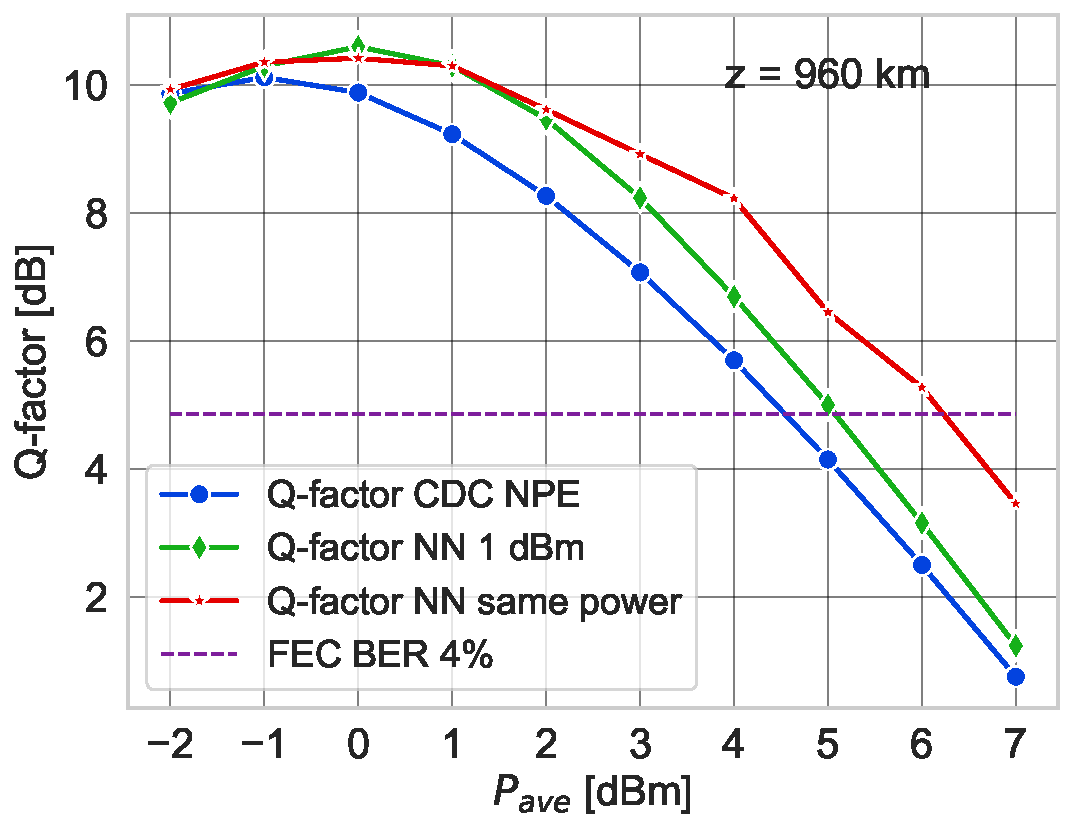
\includegraphics[width=1\linewidth]{images/nn_for_eq/q_db_vs_p_dbm_z_960_p_dbm_model_1.pdf} (a)
    }
    \end{minipage}
    \hfill
    \begin{minipage}[h]{0.48\linewidth}
    \center{
        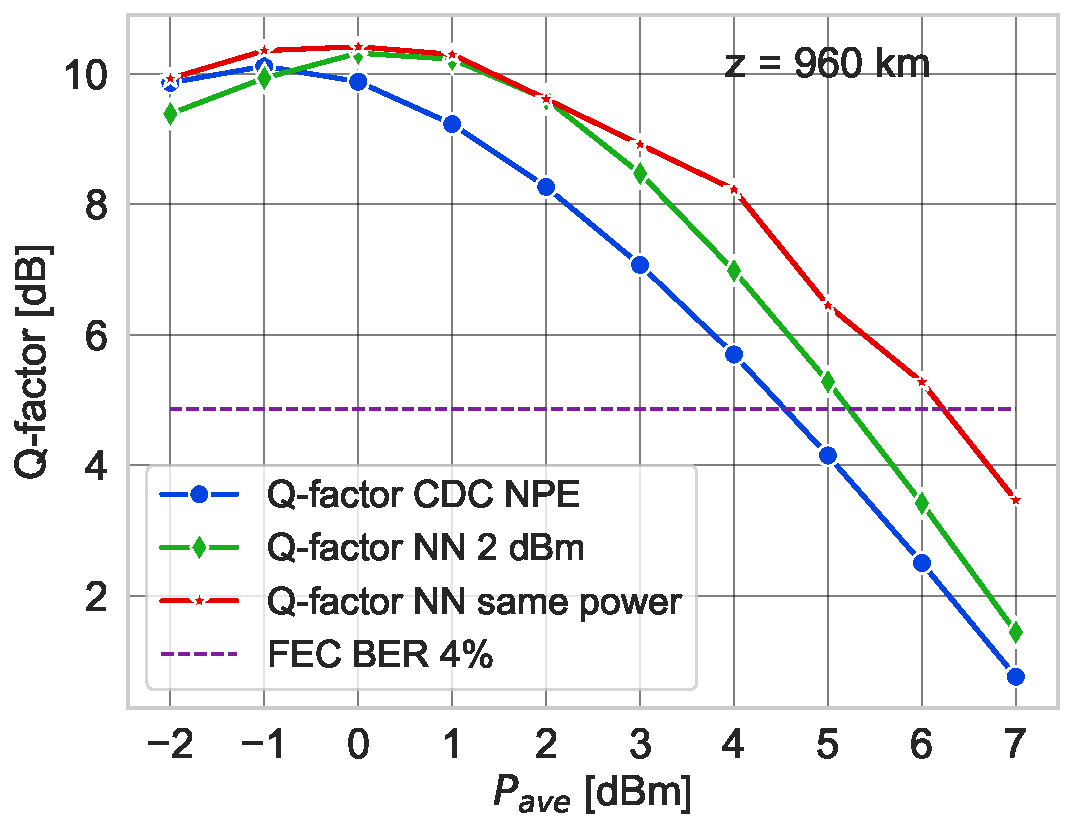
\includegraphics[width=1\linewidth]{images/nn_for_eq/q_db_vs_p_dbm_z_960_p_dbm_model_2.pdf} (b)
    }
    \end{minipage}

    \begin{minipage}[h]{0.48\linewidth}
    \center{
        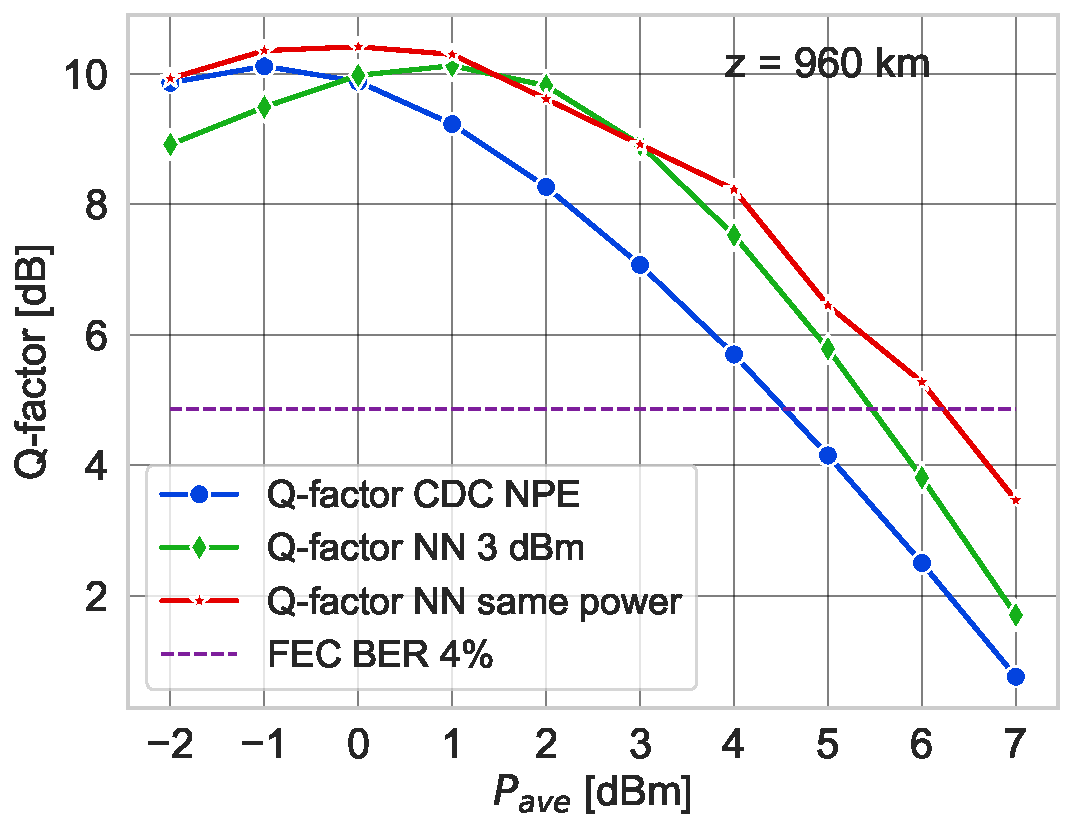
\includegraphics[width=1\linewidth]{images/nn_for_eq/q_db_vs_p_dbm_z_960_p_dbm_model_3.pdf} (c)
    }
    \end{minipage}
    \hfill
    \begin{minipage}[h]{0.48\linewidth}
    \center{
        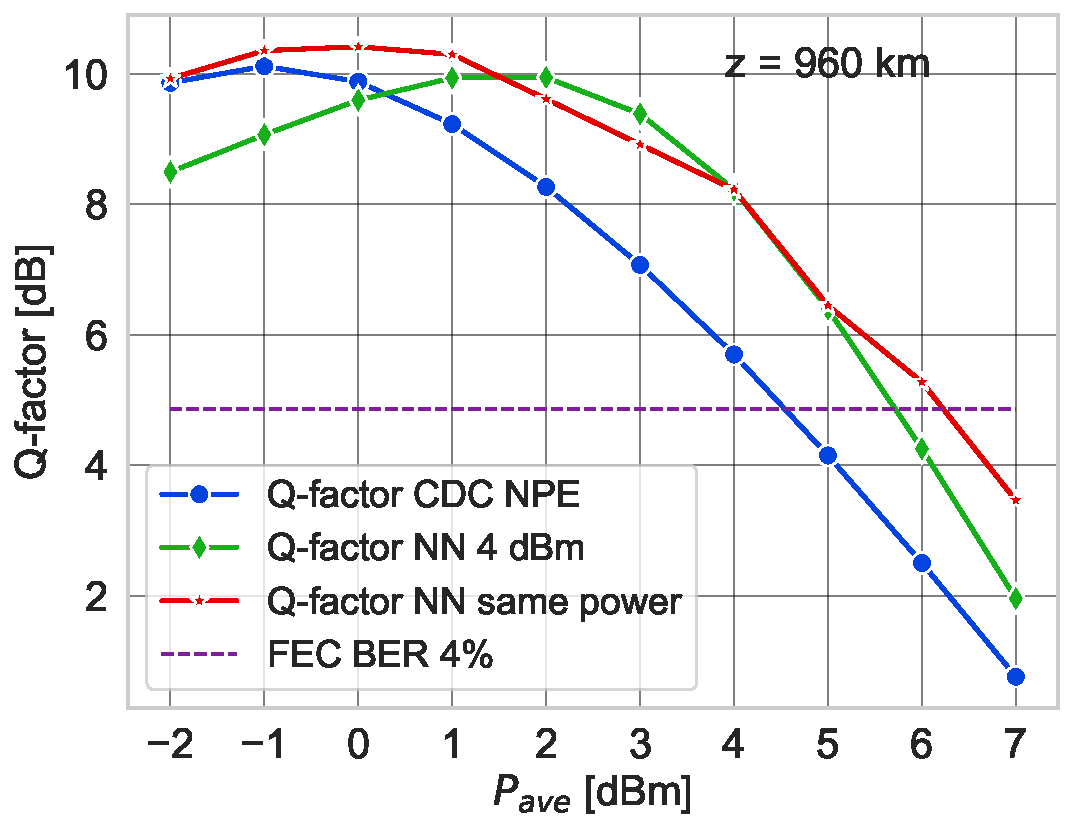
\includegraphics[width=1\linewidth]{images/nn_for_eq/q_db_vs_p_dbm_z_960_p_dbm_model_4.pdf} (d)
    }
    \end{minipage}

    \begin{minipage}[h]{0.48\linewidth}
    \center{
        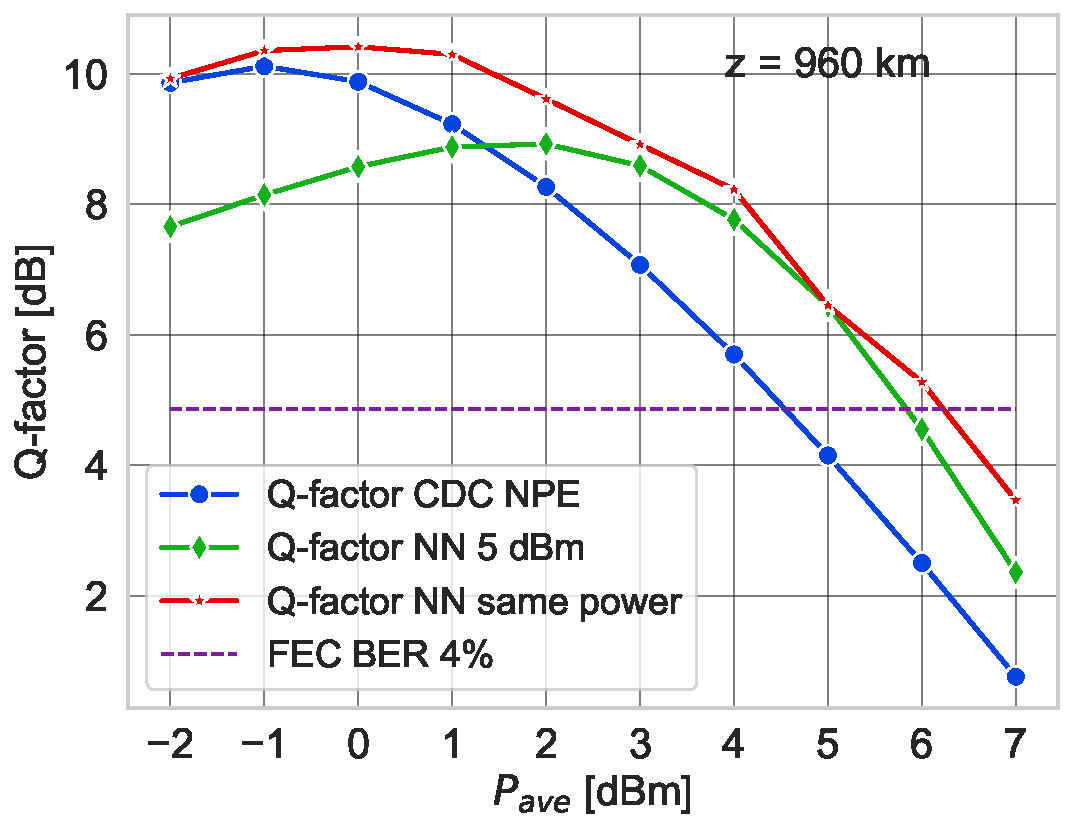
\includegraphics[width=1\linewidth]{images/nn_for_eq/q_db_vs_p_dbm_z_960_p_dbm_model_5.pdf} (e)
    }
    \end{minipage}
    \hfill
    \begin{minipage}[h]{0.48\linewidth}
    \center{
        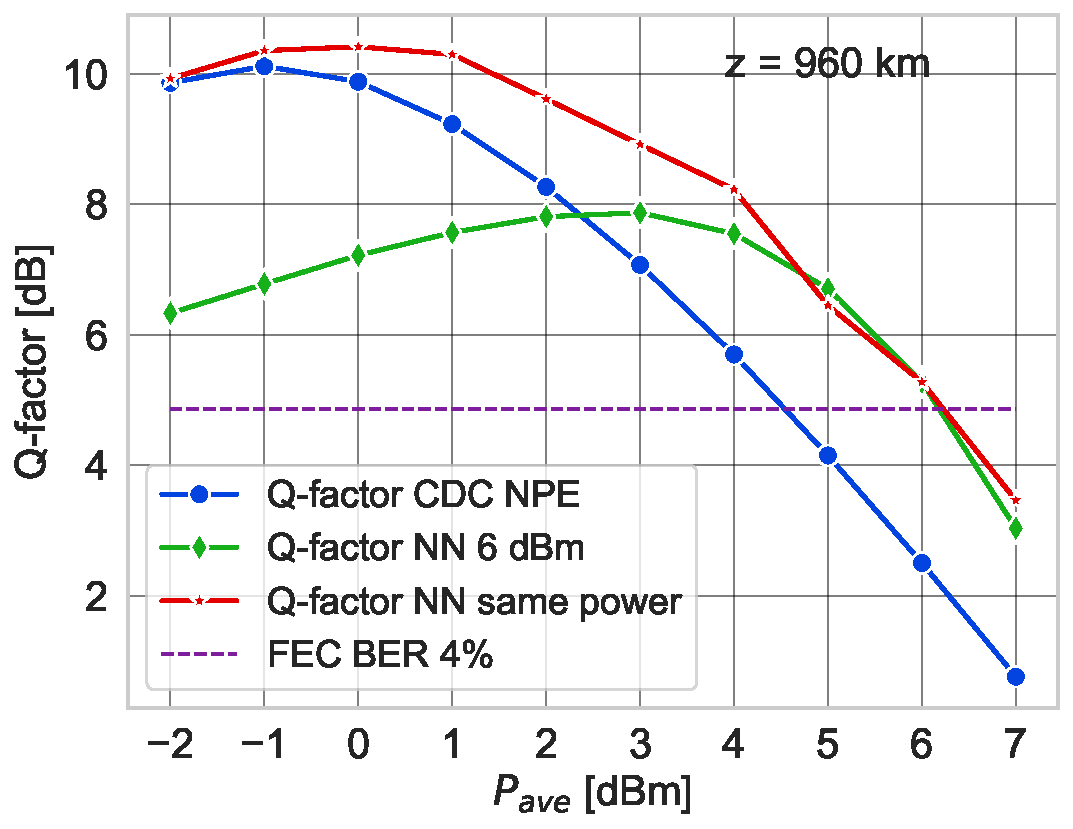
\includegraphics[width=1\linewidth]{images/nn_for_eq/q_db_vs_p_dbm_z_960_p_dbm_model_6.pdf} (f)
    }
    \end{minipage}
    \caption{Representation of dependance of Q-factor vs signal average power for different NNs trained on different signal power. It starts with 1 dBm (upper left) and subsequently increment up to 6 dBm (lower right). Propagation distance is 960 km.}
    \label{fig:nn_eq_z_960}
\end{figure}

% Figure~\ref{fig:nn_eq_z_960} representation of dependance of Q-factor vs signal average power for different NNs trained on different signal power. It starts with 1 dBm (upper left) and subsequently increment up to 6 dBm (lower right). Propagation distance is 960 km. Figure~\ref{fig:nn_eq_z_1200} represents the same for distance of 1200 km. Blue line represents Q-factor after \acrfull{cdc} and \acrfull{npe} and hard-dessicion. Red line on the graps are the same and represents the case when test power level are the same as trained. Green lines represents the performance of the model trained on specific average power level, but tested on different power level. Dashed line show 4\% BER limit for \acrlong{fec}.
% NN wich was trained with datasets with -2, -1, 0 and 7 dBm average signal power is not represented cause the performance not better than NN trained with the same power (red line) for same range of average powers and 7 dBm shows bad performance for all range except trained power.

In Figure~\ref{fig:nn_eq_z_960}, we show how the Q-factor, which measures signal quality, changes with different average signal powers for neural networks (NNs) trained at various power levels. The analysis begins with a signal power of 1 dBm (top left) and increases to 6 dBm (bottom right), over a distance of 960 km. Figure~\ref{fig:nn_eq_z_1200} presents similar data for a distance of 1200 km. In these figures, the blue line shows the Q-factor after applying \acrfull{cdc} and \acrfull{npe} followed by a hard decision process. The red line indicates the Q-factor when the NN is tested at the same power level it was trained on. The green lines show how well the NN, trained at a specific power level, performs when tested at different power levels. The dashed line marks the 4\% Bit Error Rate (BER) threshold, which is the upper limit for effective \acrlong{fec}.

NNs trained on datasets at -2, -1, 0, and 7 dBm are not included in these graphs because their performance did not exceed that of NNs trained at the same power levels (red line). Furthermore, the NN trained at 7 dBm did not perform well across the power range, except precisely at the trained power level.


% Figure~\ref{fig:nn_eq_z_960} show us that NN can significantly improve performance after equalisation. Across different regimes, NN can show more than 2 dB improvement (Fig.~\ref{fig:nn_eq_z_960}d, 4 dBm) and even can shift system beyond the \acrshort{fec} line like on Fig.~\ref{fig:nn_eq_z_960}f for 5 and 6 dBm. Another interesting result is that NN performance are not limited with one trained power. For example, Fig.~\ref{fig:nn_eq_z_960}c NN trained on 3 dBm, shows good performance (comarable with NN trained on the same power) for 1 and 2 dBm test power level. Even more interesting that NN trained on 4 dBm performes better than NN trained on the same power for 2 and 3 dBm test power (Fig.~\ref{fig:nn_eq_z_960}d). It means that even without transfer learning and fine tuning NN ``understand'' the effect on nonlinearity and can succefully predict correction $\eta_k$. Why it is important? Because it means that NN not limited for specific power and can be used for different types of systems and regimes without training process. Next step for future research is to apply transfer learning (explain what is it) where we can make even more wide scenarious for training.

Figure~\ref{fig:nn_eq_z_960} illustrates that neural networks (NNs) can markedly enhance signal quality post-equalization. In various conditions, NNs have achieved more than a 2 dB improvement in performance, as seen in Fig.~\ref{fig:nn_eq_z_960}d for 4 dBm signals. Impressively, they can even push system performance beyond the forward error correction (FEC) threshold, as depicted for 5 and 6 dBm in Fig.~\ref{fig:nn_eq_z_960}f.

An additional noteworthy finding is the versatility of NNs across different power levels. For instance, an NN trained on a 3 dBm signal can effectively improve performance for 1 and 2 dBm test power levels, as shown in Fig.~\ref{fig:nn_eq_z_960}c. Remarkably, an NN trained on 4 dBm outperforms an NN trained at the same power for test powers of 2 and 3 dBm, as observed in Fig.~\ref{fig:nn_eq_z_960}d. This suggests that NNs can generalize the impact of nonlinearity and accurately predict the necessary corrections $\eta_k$. The significance of this is that NNs are not confined to a single power level and can be adapted to various system types and operating conditions without a new training phase.

A future research direction is to implement transfer learning, which is a method where a model developed for one task is reused as the starting point for a model on a second task. This approach could broaden the range of scenarios for NN training, enhancing their adaptability and efficiency.



\begin{figure}[tpb]
    \begin{minipage}[h]{0.48\linewidth}
    \center{
        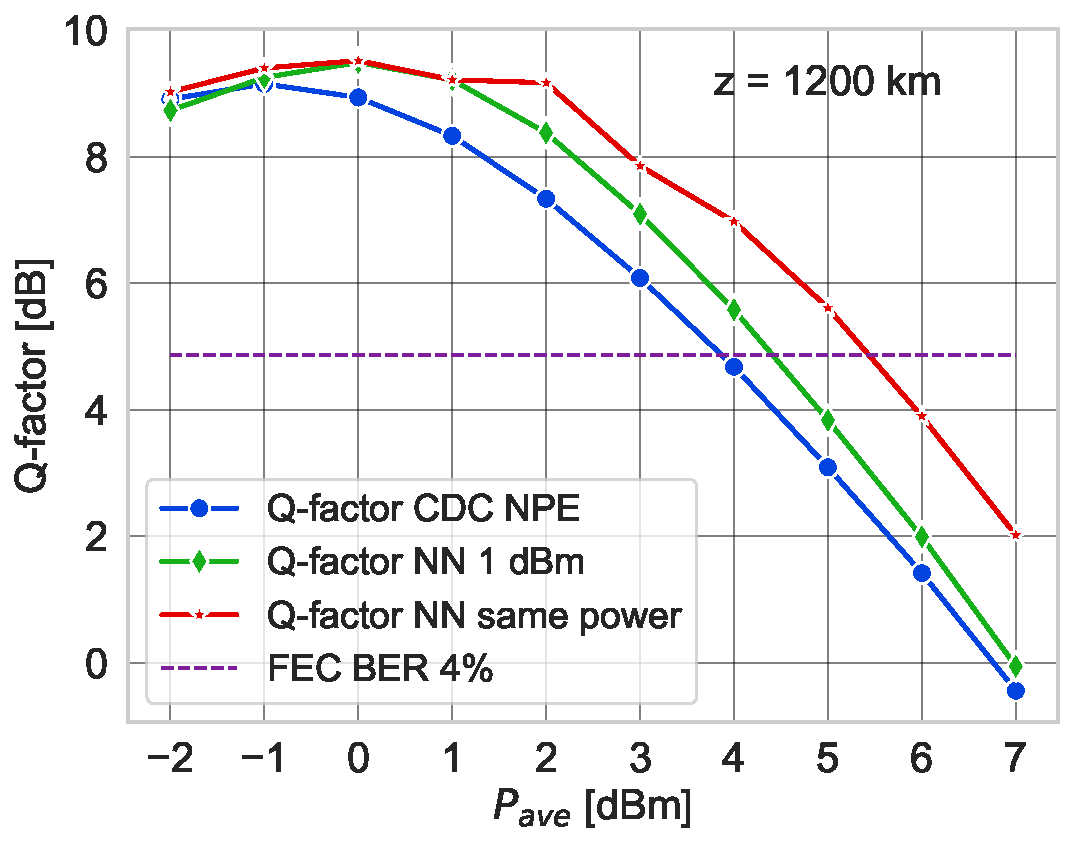
\includegraphics[width=1\linewidth]{images/nn_for_eq/q_db_vs_p_dbm_z_1200_p_dbm_model_1.pdf} (a)
    }
    \end{minipage}
    \hfill
    \begin{minipage}[h]{0.48\linewidth}
    \center{
        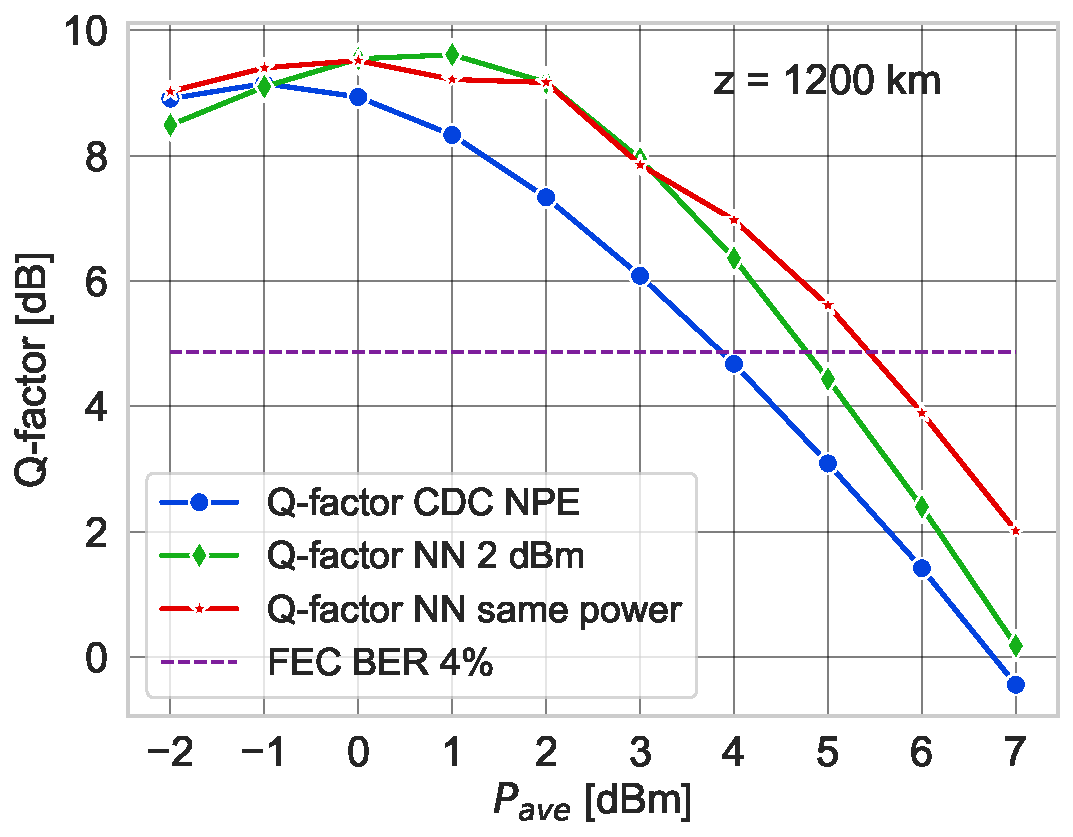
\includegraphics[width=1\linewidth]{images/nn_for_eq/q_db_vs_p_dbm_z_1200_p_dbm_model_2.pdf} (b)
    }
    \end{minipage}

    \begin{minipage}[h]{0.48\linewidth}
    \center{
        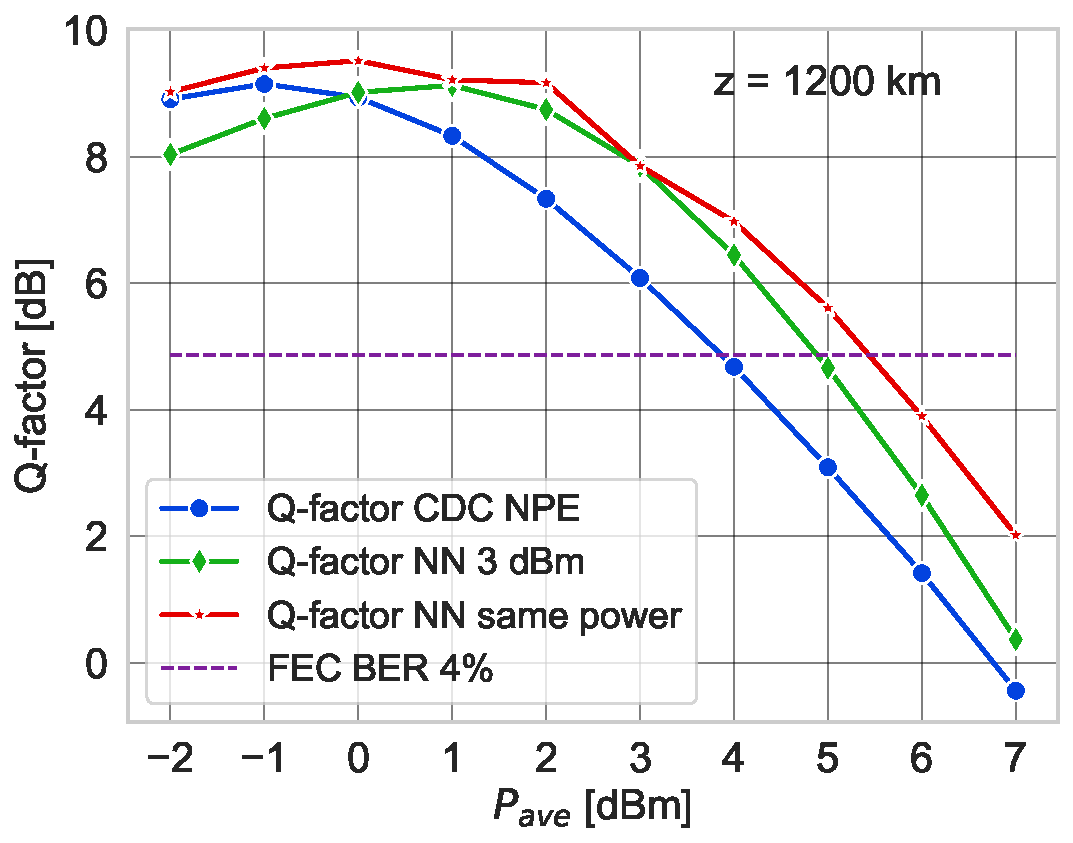
\includegraphics[width=1\linewidth]{images/nn_for_eq/q_db_vs_p_dbm_z_1200_p_dbm_model_3.pdf} (c)
    }
    \end{minipage}
    \hfill
    \begin{minipage}[h]{0.48\linewidth}
    \center{
        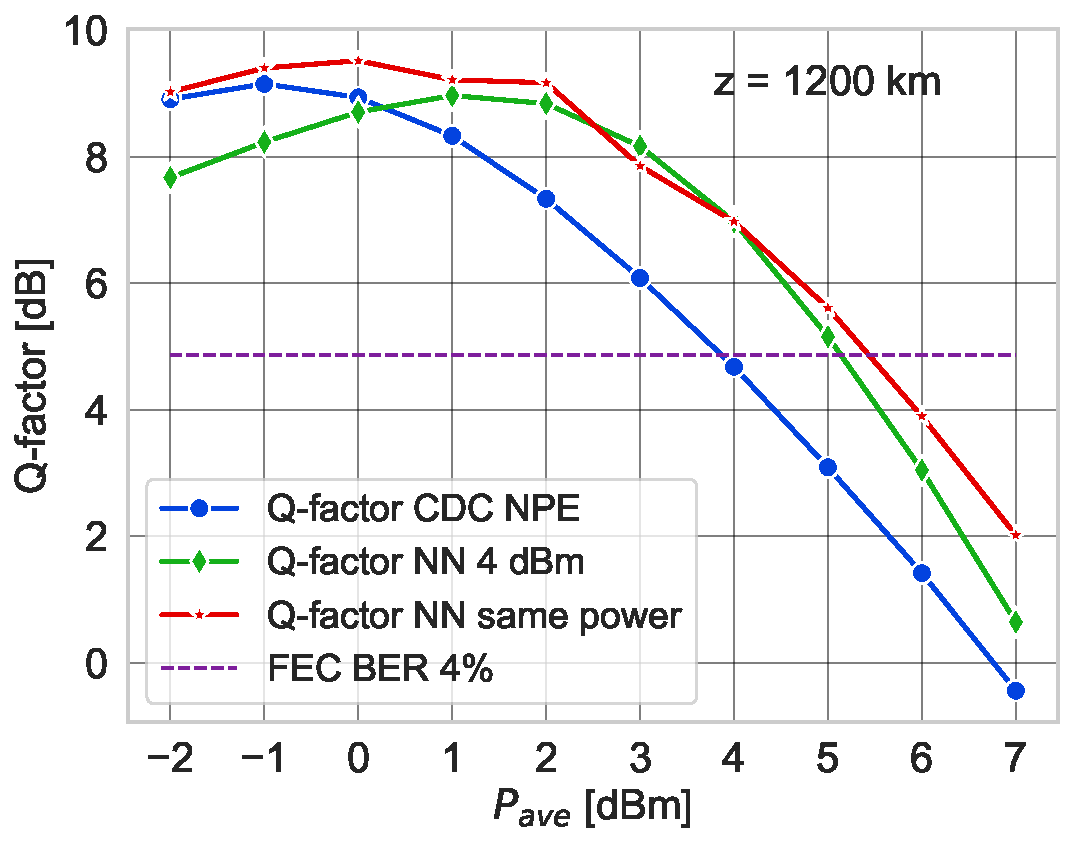
\includegraphics[width=1\linewidth]{images/nn_for_eq/q_db_vs_p_dbm_z_1200_p_dbm_model_4.pdf} (d)
    }
    \end{minipage}

    \begin{minipage}[h]{0.48\linewidth}
    \center{
        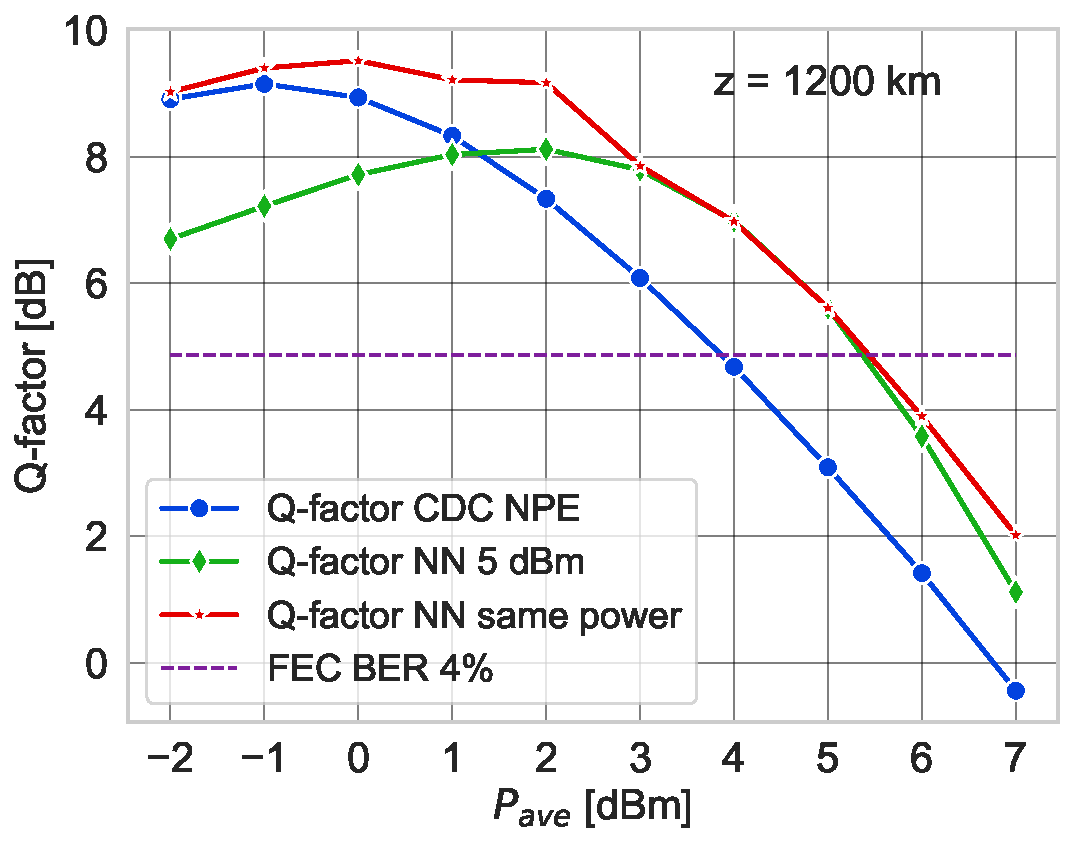
\includegraphics[width=1\linewidth]{images/nn_for_eq/q_db_vs_p_dbm_z_1200_p_dbm_model_5.pdf} (e)
    }
    \end{minipage}
    \hfill
    \begin{minipage}[h]{0.48\linewidth}
    \center{
        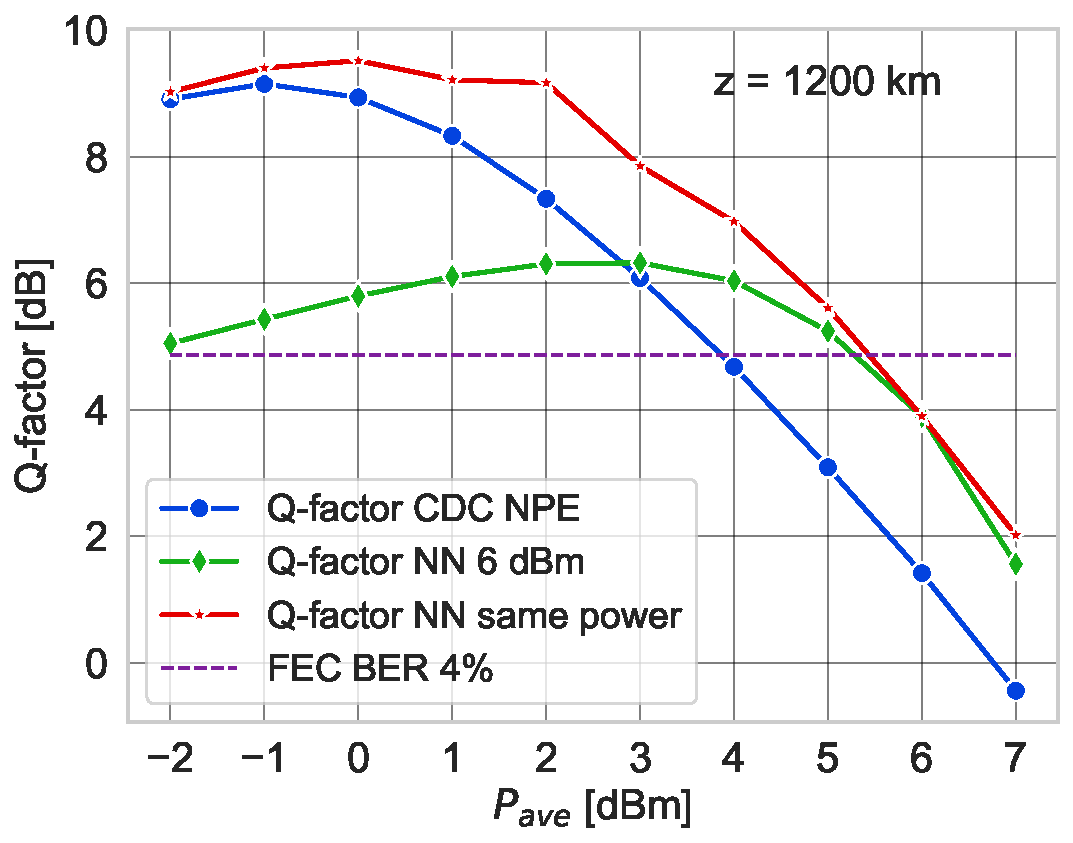
\includegraphics[width=1\linewidth]{images/nn_for_eq/q_db_vs_p_dbm_z_1200_p_dbm_model_6.pdf} (f)
    }
    \end{minipage}
    \caption{Representation of dependance of Q-factor vs signal average power for different NNs trained on different signal power. It starts with 1 dBm (upper left) and subsequently increment up to 6 dBm (lower right). Propagation distance is 1200 km.}
    \label{fig:nn_eq_z_1200}
\end{figure}

% Figure~\ref{fig:nn_eq_z_1200} shows a bit other but similar picture. NN can succesfully perform nonlinear equalisation task and improve system performance. For all trained powers on  Fig.~\ref{fig:nn_eq_z_1200} we see NN can shift Q-factor level to acceptable region for \acrshort{fec} (upper dashed line). But the difference from Fig.~\ref{fig:nn_eq_z_960} which are remarkable is that NN trained for specific power almost never outperform NN trained on the same power as test power. It means that for this amount of nonlinear effects (it is additional 3 spans of fiber) we need to expand our approach to receive NN which capable to perform in different power regimes (we can still see good performance on Fig.~\ref{fig:nn_eq_z_1200}e where green line for 3 and 4 dBm almost coincide with red one). 


% As a final remark, I want to stress that this is an demonstration of possible neural network utilisation for future research. It showed that data-driven approach can be very fruitful if we have enough data. With HpCom simulator now the data for various types of fibres and power levels can be calculated very fast and easy. This results will be a part of the overview article about machine learning utilisation for nonlinear equalisation which currently in work and beyond the scope of this thesis.

In Figure~\ref{fig:nn_eq_z_1200}, we see a pattern similar to the one in Figure~\ref{fig:nn_eq_z_960}. Neural networks (NNs) effectively perform nonlinear equalization, enhancing system performance. For all power levels examined, NNs managed to raise the Q-factor to levels suitable for forward error correction (FEC), as shown by surpassing the upper dashed line in Fig.~\ref{fig:nn_eq_z_1200}. However, a noticeable difference is that NNs specialized for a certain power level generally do not exceed the performance of NNs trained and tested at the same power level. This implies that with the added complexity from three extra spans of fiber, our current method needs to be improved to create NNs that are versatile across various power conditions (although Fig.~\ref{fig:nn_eq_z_1200}e shows promising results where the green line for 3 and 4 dBm nearly matches the red line).

To conclude, the results presented here are an example of how NNs can be leveraged in future research. They demonstrate that a data-driven approach can be highly effective when sufficient data is available. Thanks to the HpCom simulator, data generation for different types of fibers and power levels is now quicker and easier. These findings will contribute to an upcoming review article on the application of machine learning in nonlinear equalization, which is currently in progress and will extend beyond the scope of this thesis.
